\chapter{Results}

\section{Comparison With Literature Values} %TODO: https://physics.nist.gov/cgi-bin/cuu/Value?alph for fsc, https://link.springer.com/article/10.1007/BF00617498 for carrier density
\subsection{Charge Carrier Density}
\begin{figure}
	\centering
	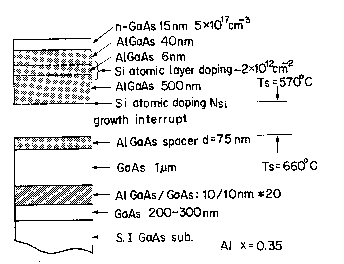
\includegraphics[width=.5\textwidth]{./img/sakuccd.pdf}
	\caption[Epitaxial layer sequence comparison]{\textbf{Epitaxial layer sequence as used in \cite{ccd}}}
	\label{fig:sakuccd}
\end{figure}
The carrier concentrations found in \autoref{sec:ccd} do not lie close to values found in \cite{ccd}.
Saku et al. find carrier densities in the order of \SI{3e11}{\per\centi\meter\squared} at temperatures of around \SI{4}{\kelvin}.
They use modulation-doped AlGaAs-GaAs heterostructures with similar epitaxial layer sequences as in this experiment, shown in \autoref{fig:sakuccd}.

\subsection{Fine-structure constant}
Comparing the values found for the fine-structure constant in \autoref{sec:fine} with literature values in \cite{NIST} confirms the plausibility of the results.
However, the literature value only lies within the error boundaries for the value found at \SI{2}{\kelvin} and \SI{100}{\micro\ampere} ($\alpha^{-1}_{\SI{2}{\kelvin},\SI{100}{\micro\ampere}} = \num{142.43(578)}$), featuring a relative deviation of \num{3.93}\%.

\section{Sources of Error} %TODO: Hot spots? --> iNvEsTiGaTe!!!
